\section{Course Pages}

The main aspects that the features of the course pages that will be analysed and discussed are:
\begin{itemize}
    \item Functional Requirements - have the features outlined been completed?
    \item Non-functional Requirements - how well do the features complete their objectives?
    \item Usability Tests - how do users utilise the features and what do they think of it?
\end{itemize}

\subsection{Functional Requirements}
As stated before, there were a total of 14 functional requirements. Within these requirements there were 6 high priorty requirements, 3 medium priority requirements and 5 low priority requirements.
In total only 9 of the functional requirements were completed. The 5 features that were not complete due to being low priority.

\subsubsection{Completed}
\begin{itemize}
    \item Users can click on the links in the sidebar to be directed to the corresponding component;
    \item Users can view the announcments within the dashboard;
    \item Users can view the course content;
    \item Administrators of the course can create announcments within the dashboard;
    \item Users can make comments on announcments;
    \item Administrators can upload the course outline onto the course outline page;
    \item Users can download the course content;
    \item Administrators can edit the sidebar to change what components are linked;
    \item Course content is catergorised based on how the content is catergorised in the topic tree;
    \item Administrators can edit the announcements made in the dashboard;
    \item Users can intereact with widgets to enchance their experience with the LMS;
    \item Users can toggle on or off specific widgets.
\end{itemize}

\subsubsection{Uncompleted}
\begin{itemize}
    \item Users can view the course outline of a course;
    \item Administrators can add course content into the page by selecting content from the topic tree;
    \item Administrators can upload the course outline onto the course outline page;
    \item Administrators can edit the sidebar to change what components are linked;
    \item Users can toggle on or off specific widgets.
\end{itemize}

The course outline feature was removed from the final design as it was not highly prioritised and other features being prioritised. 
The feature for administrators to add course content onto a course was streamlined, so that administrators can add content on the topic tree and have those changes be reflected on the course content page.
The last feature that was not complete was the functionality of allowing users to toggle on or off specific widgets. This was due to the lack of priority for this feature and thus was not implemented.\\

Apart from the outlined requirements, there were also other functionality that were introduced:
\begin{itemize}
    \item Users can view the courses that they are enrolled in;
    \item Users can select a course that they would want to view the course pages for;
    \item Users can view the most recent announcement;
    \item Users can view the progress of their courses;
\end{itemize}

These functional features were added early in Thesis B as they are the features that would make up the course selection page.

\subsection{Non-Functional Requirements}
The non-functional requirements that will be used to analyse the course pages are:
\begin{itemize}
    \item Performance;
    \item Accessibility.
    \item Responsiveness;
\end{itemize}

\subsubsection{Performance}
Google Lighthouse was utilised to quantify the performance of the different aspects within the course pages. Google Lighthouse provides a simple way to test various aspects of a page,
 for example the performance, accessibility and assessing whether the website complies with best practices.
The course pages that will be analysed are comprised of:
\begin{itemize}
    \item Course selection page;
    \item Course dashboard.
    \item Course content page;
\end{itemize}

The performance of all of these pages all range within 40-50, indicating that there are a variety of further optimisations to better the performance of each page.

\begin{figure}[h!]
    \centering
    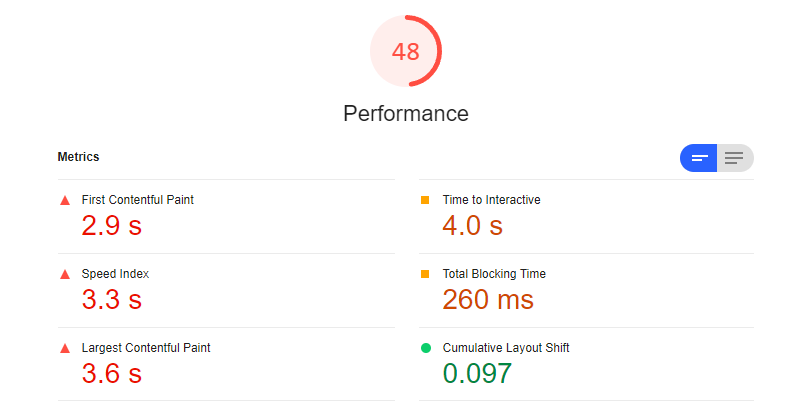
\includegraphics[scale=0.4]{course-selection-performance}
    \caption{Performance report of the course selection page}
\end{figure}

\begin{figure}[h!]
    \centering
    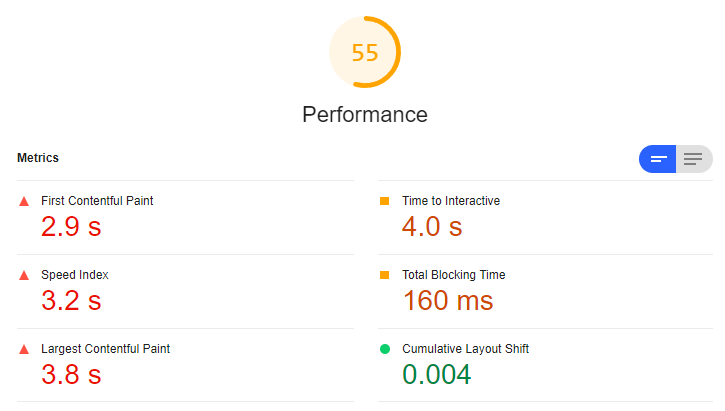
\includegraphics[scale=0.4]{course-dashboard-performance}
    \caption{Performance report of the course dashboard page}
\end{figure}

\begin{figure}[h!]
    \centering
    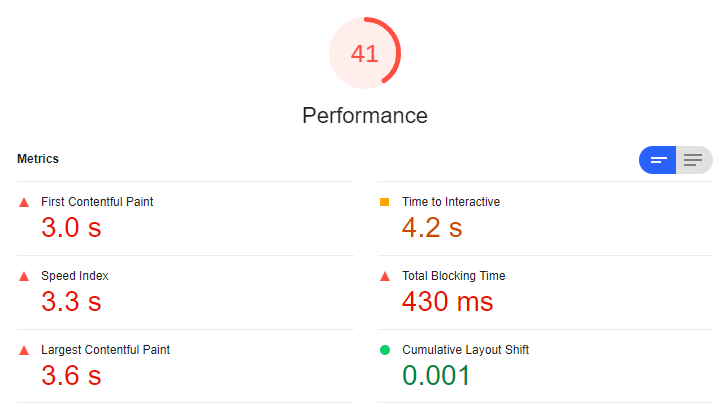
\includegraphics[scale=0.4]{content-page-performance}
    \caption{Performance report of the course content page}
\end{figure}

As shown, the performance of the course selection page is 48/100, the course dashboard being 55/100 and the course content page being 41/100. This would be due to the variety of features within the page which would require numerous API calls.
Possible optimisations could include, restructuring the use of API calls and database schema to improve fetch times and also minifying javascript files which would further improve performance as this test was run on a development server.
For the course selection page, there are a variety of features, such as the most recent announcement, course progress or most recently accessed topic. This page could be optimised by having the associated data be attached to a user, making only 1 API call needed.
The course dashboard involves a variety of API calls, which include getting the announcement data, the user who made the announcement and other metadata. 
The course pages can be improved through redesigning the topic schema. The main concern was the multiple API calls needed to get the topic data and the corresponding files. If a topic contained a large file, then the API call to get the topic data would take longer.

\subsubsection{Accessibility}
\begin{figure}[h!]
    \centering
    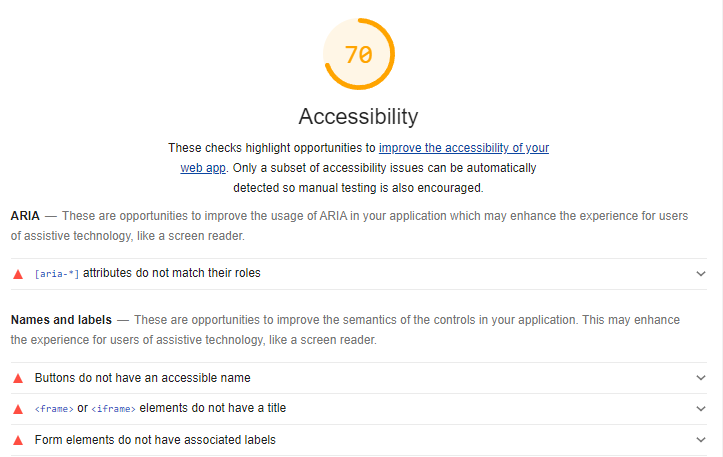
\includegraphics[scale=0.4]{course-selection-accessibility}
    \caption{Accessibility report of the course selection page}
\end{figure}

\begin{figure}[h!]
    \centering
    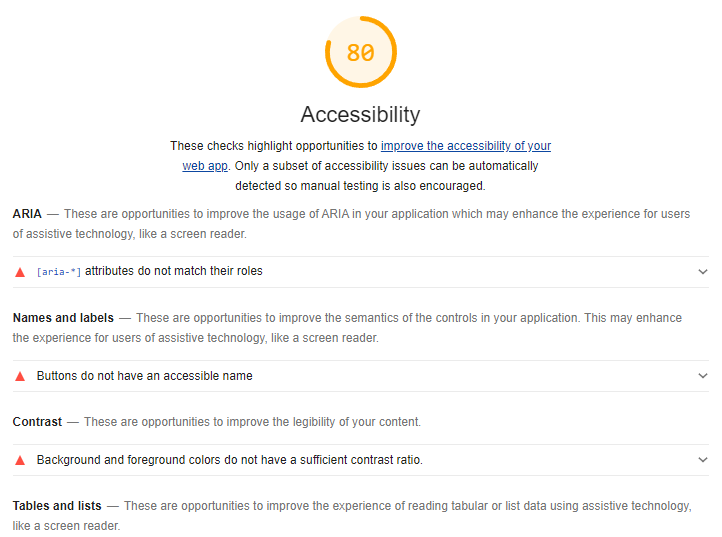
\includegraphics[scale=0.4]{course-dashboard-accessibility}
    \caption{Accessibility report of the course dashboard page}
\end{figure}

\begin{figure}[h!]
    \centering
    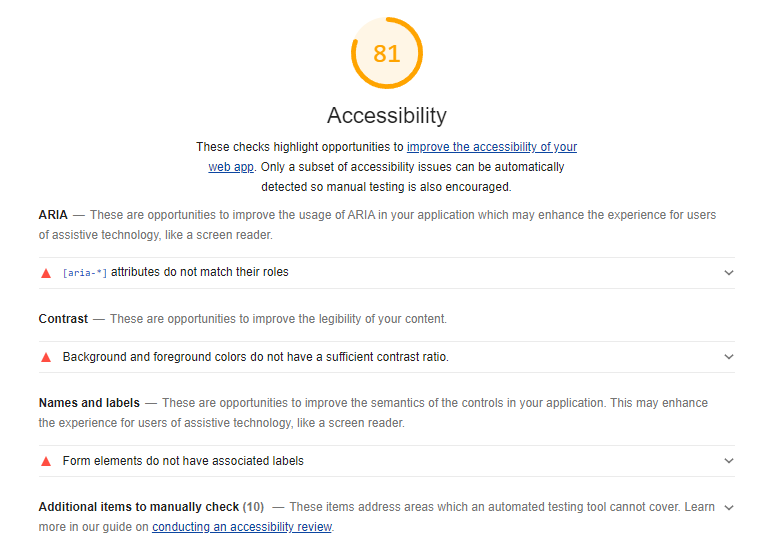
\includegraphics[scale=0.4]{content-page-accessibility}
    \caption{Accessibility report of the course content page}
\end{figure}

As shown the accessibility of the course pages range within 70-80 and as such is one aspect that could be improved on with minor changes. With the use of Chakra UI, many aspects of accessbility within frontend design was already handled. For example aria labels and the roles of certain HTML elements were handled with Chakra UI.
However some aspects such as colour contrast and certain HTML semantics can be improved. For example some buttons do not have accessible names for screen readers to be able to read.

\subsubsection{Responsiveness}
The responsiveness of the course pages were one aspect of design that was deliberately designed. Each page has 3 intermediate stages, which correspond to screen widths, with the breakpoints being 990px and 765px.
The main aspect of responsiveness is to provide the same functionality regardless of the screen size. This however has not been fully achieved within the course pages.
The corresponding component affecting the responsiveness are the 2 sidebars, the navigation sidebar and widgets bar. As shown in the figures, the medium and small screen sizes do not have any widget functionality.


\begin{figure}[h!]
    \centering
    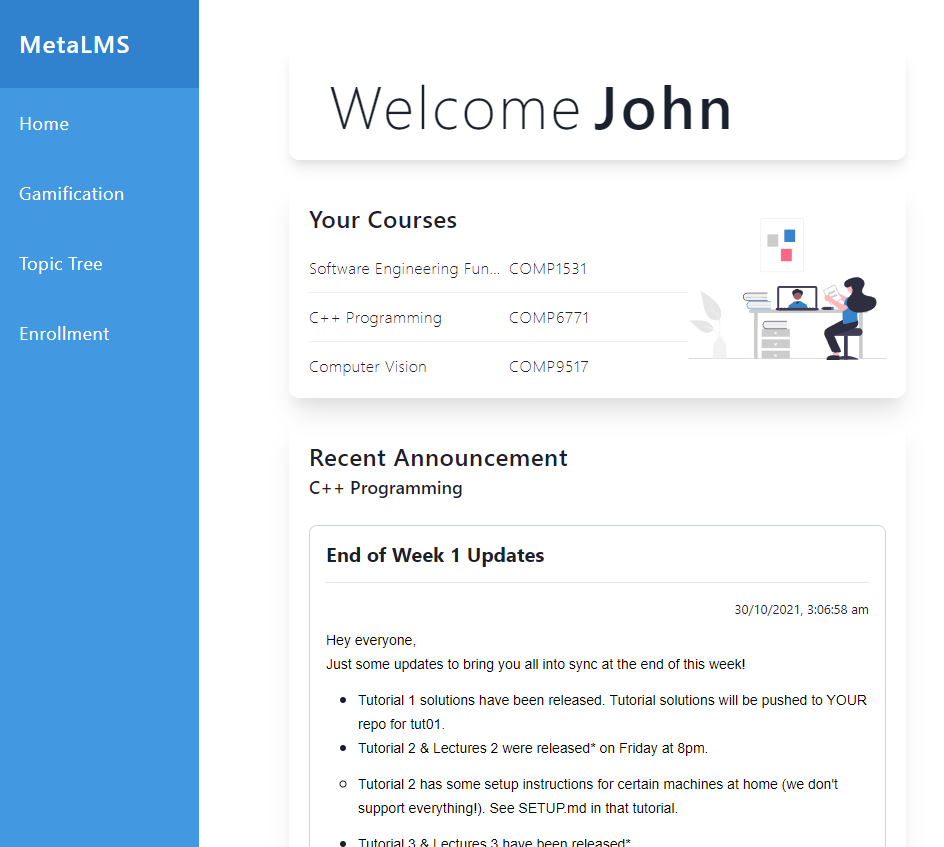
\includegraphics[scale=0.4]{course-selection-medium}
    \caption{Medium screen size for the course selection page}
\end{figure}

\begin{figure}[h!]
    \centering
    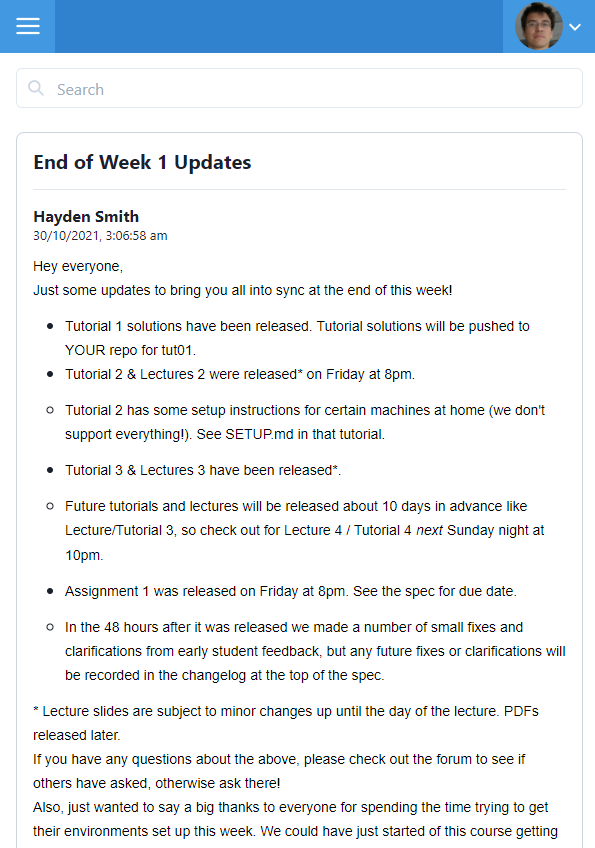
\includegraphics[scale=0.4]{course-dashboard-small}
    \caption{Small screen size for the course dashboard page}
\end{figure}

A way to provide this functionality would be to allow users to select an option when clicking on the account button on the top right of the screen which would open up the widgets bar.
In this design, the functionality of the widgets bar would still be present within smaller screens and also larger screens, however is less accessible for users to navigate.

\subsection{Usability Tests}

The usability tests were conducted on a variety of UNSW students primarily studying computer science and engineering.
For the usability testing a series of tasks were utilised to simulate several use cases for regular users and administrators.
The following tasks were presented to the individuals in which the usability tests were conducted on:
\begin{enumerate}
    \item Login as john smith.
    \item Can you tell me what courses you are enrolled in?
    \item Can you tell me the progress of the courses?
    \item Can you identify anything else that is shown on the page?
    \item Can you make a reminder on the calendar and delete it?
    \item Can you tell me what the reminder section is for and what do you think of it?
    \item Go to the C++ programming course home page and to the content of that course.
    \item Can you find and open the while loops pdf file and signify that you have completed it?
    \item Tell me the perquisites of the topic that the while loops pdf file is in.
    \item On the same page can you navigate to another course?
    \item Login as jane doe.
    \item Can you identify what is shown on the page?
    \item Go the C++ Programming page and create an announcement with the title: ‘Week 2 updates’ and content: ‘Continue with your work and finish variable topic content for next week’.
    \item Edit the newly created announcement so the content is ‘Finish while loops content this week and next week we will announce a new assignment’.
    \item Delete the announcement.
\end{enumerate}

Before beginning each individual usability test, each participant was given context of the topic groups, topics and topic files. Specifically the relationship between courses and topic groups were explained, along with how topics contain 4 types of material (preparation, content, practice, assessments).
Most users could navigate through all of the tasks with ease. However there were certain aspects that took longer than expected to complete or did not fully understand.
These were:
\begin{itemize}
    \item Not understanding the which announcement is for which particular course in the course selection page
    \item Not understanding the most recently accessed feature
    \item Not noticing the difference between the course selection page and course dashboard/content page.
    \item Difficulty to distinguish the separate topics and content types in the course content page
\end{itemize}

These results highlight UI deficiency in providing a clear outline of allowing users to understand the functionality.
For the first 2 points, help buttons or tooltips could be implemented to provide the user with the ability to search how the feature is intended to be used.
The 3rd point involves the lack of unique distinction between the course selection and a particular course page. A possible solution would be to change the side bar colors when a user enters a particular course page.
This would be similiar to WebCMS3 as it uses colours to distinguish different courses from each other.
Another supplement to this solution to provide more distinction that a user can return back to the course selection page would be to highlight the return button.
Lastly the accordion within the course content page would need to be updated to further distinguish items within a topic. This can be done by increasing the margin for each item or having different font weights for topics or topic content.
In general the course dashboard had no complaints as it was a familiar feature for users to utilise.
Some users also conveyed some concern with understanding the relationship between topic groups and courses, as they would not have understood how to utilise the MetaLMS without the background context.
In this aspect, the MetaLMS would benefit with a general help page to assist users with understanding the several relationships.